\documentclass{beamer}

% --- Escolha de Tema e Cores ---
\usetheme{Madrid} % Um tema popular e limpo. Outras opções: Boadilla, AnnArbor, Warsaw
\usecolortheme{default}

% --- Pacotes e Configurações ---
\usepackage[utf8]{inputenc}
\usepackage{graphicx}
\usepackage{amsmath}

% --- Informações do Título ---
\title[Análise de Dependências Go]{Gestão de Dependências em Projetos Go com Ordenação Topológica}
\author{Nicholas Pereira Cristófaro \and Marcos Campos Dias}
\institute{Pontifícia Universidade Católica de Minas Gerais (PUC Minas)}
\date{Trabalho Prático - Processamento de Dados com Grafos - 2025}

% --- Início do Documento ---
\begin{document}

% ---------------------------------------------------------------
% SLIDE 1: Título
% ---------------------------------------------------------------
\begin{frame}
  \titlepage
\end{frame}

% ---------------------------------------------------------------
% SLIDE 2: Introdução e Motivação
% ---------------------------------------------------------------
\begin{frame}
  \frametitle{Introdução: O Problema das Dependências}

  \begin{columns}[T] % Divide o slide em colunas
    \begin{column}{0.6\textwidth}
      \textbf{O Desafio:}
      \begin{itemize}
        \item A gestão de dependências em software moderno é complexa ("inferno de dependências").
        \item Em Go, a ordem de inicialização de pacotes é crítica e estrita.
        \item \alert{Dependências Cíclicas} são erros de compilação, pois impedem a determinação de uma ordem de inicialização válida.
      \end{itemize}
    \end{column}
    \begin{column}{0.4\textwidth}
        \centering
        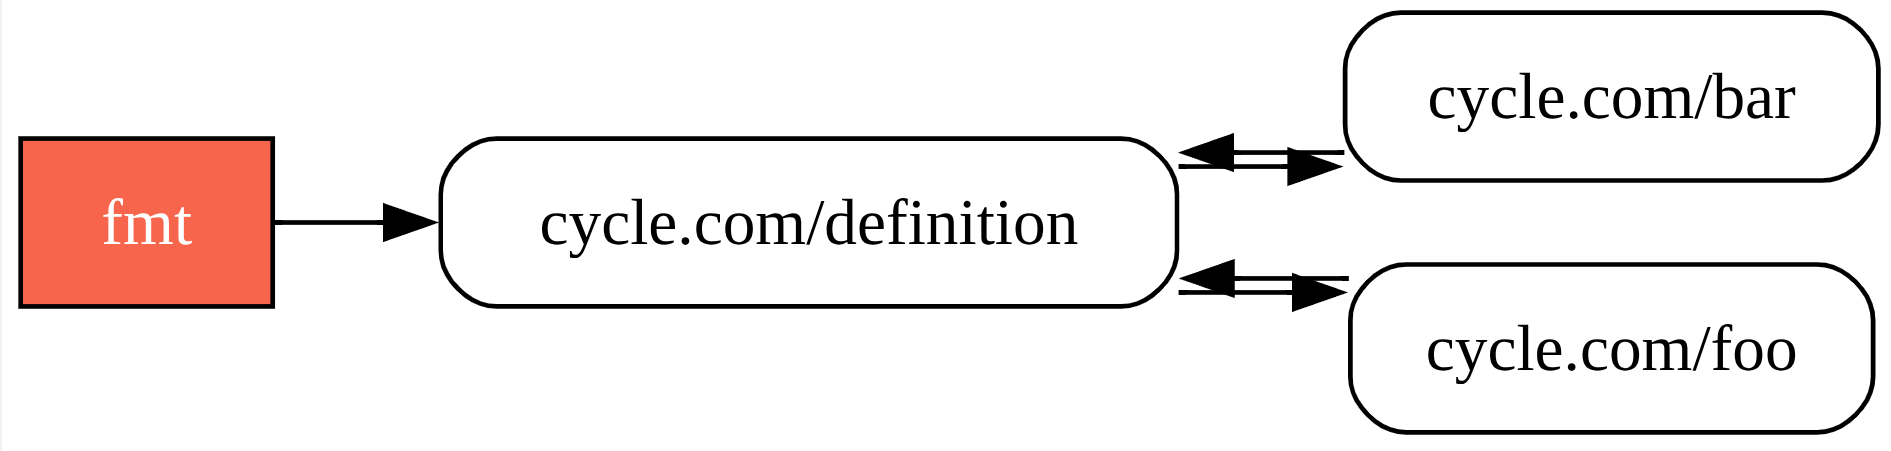
\includegraphics[width=\textwidth]{images/cycle.png}
        \tiny
        \textit{Um ciclo impede a ordenação.}
    \end{column}
  \end{columns}
\end{frame}

\begin{frame}
  \frametitle{Introdução: O Problema das Dependências}
      \textbf{Nossa Proposta:}
      \begin{itemize}
        \item Uma ferramenta que modela as dependências de projetos Go como um grafo direcionado.
        \item Utiliza a \alert{Ordenação Topológica} para:
        \begin{itemize}
          \item Determinar a sequência de compilação segura.
          \item Visualizar a arquitetura do projeto.
        \end{itemize}
      \end{itemize}
\end{frame}


% ---------------------------------------------------------------
% SLIDE 3: Metodologia
% ---------------------------------------------------------------
\begin{frame}
  \frametitle{Metodologia: Grafos e Ordenação Topológica}

  \textbf{1. Modelagem do Problema}
  \begin{itemize}
    \item Cada \textbf{pacote Go} é um \textbf{vértice} no grafo.
    \item Cada diretiva \texttt{import} de um pacote A para um pacote B cria uma \textbf{aresta direcionada} de B para A ($B \rightarrow A$), significando "A depende de B".
  \end{itemize}
  \vspace{1cm}

  \textbf{2. Solução com Ordenação Topológica}
  \begin{itemize}
    \item É uma ordenação linear dos vértices onde cada dependência aparece antes do pacote que a utiliza.
    \item \alert{Só é possível se o grafo for um DAG} (Grafo Acíclico Direcionado).
    \item O resultado é a ordem de compilação/inicialização segura dos pacotes.
  \end{itemize}

\end{frame}

% ---------------------------------------------------------------
% SLIDE 4: Algoritmo de Kahn
% ---------------------------------------------------------------
\begin{frame}
    \frametitle{O Algoritmo de Kahn (Visão Geral)}

    A ordenação é feita em camadas, de forma iterativa:

    \begin{enumerate}
        \item \textbf{Calcular Grau de Entrada:} Contar quantas dependências cada pacote (nó) possui.
        \vspace{0.5cm}
        \item \textbf{Encontrar as Raízes:} Iniciar com uma fila de todos os pacotes que não têm dependências (grau de entrada zero).
        \vspace{0.5cm}
        \item \textbf{Processar em Camadas:}
            \begin{itemize}
                \item Remover um pacote da fila e adicioná-lo à lista ordenada.
                \item "Dar baixa" nessa dependência para todos os pacotes que a importavam.
                \item Se algum desses pacotes ficar com grau de entrada zero, adicioná-lo à fila.
            \end{itemize}
        \vspace{0.5cm}
        \item \textbf{Verificar Ciclos:} Se, ao final, nem todos os pacotes foram para a lista ordenada, o grafo possui um ciclo.
    \end{enumerate}
\end{frame}

% ---------------------------------------------------------------
% SLIDE 5: Arquitetura da Ferramenta
% ---------------------------------------------------------------
\begin{frame}
  \frametitle{Arquitetura da Ferramenta}

  \begin{figure}
    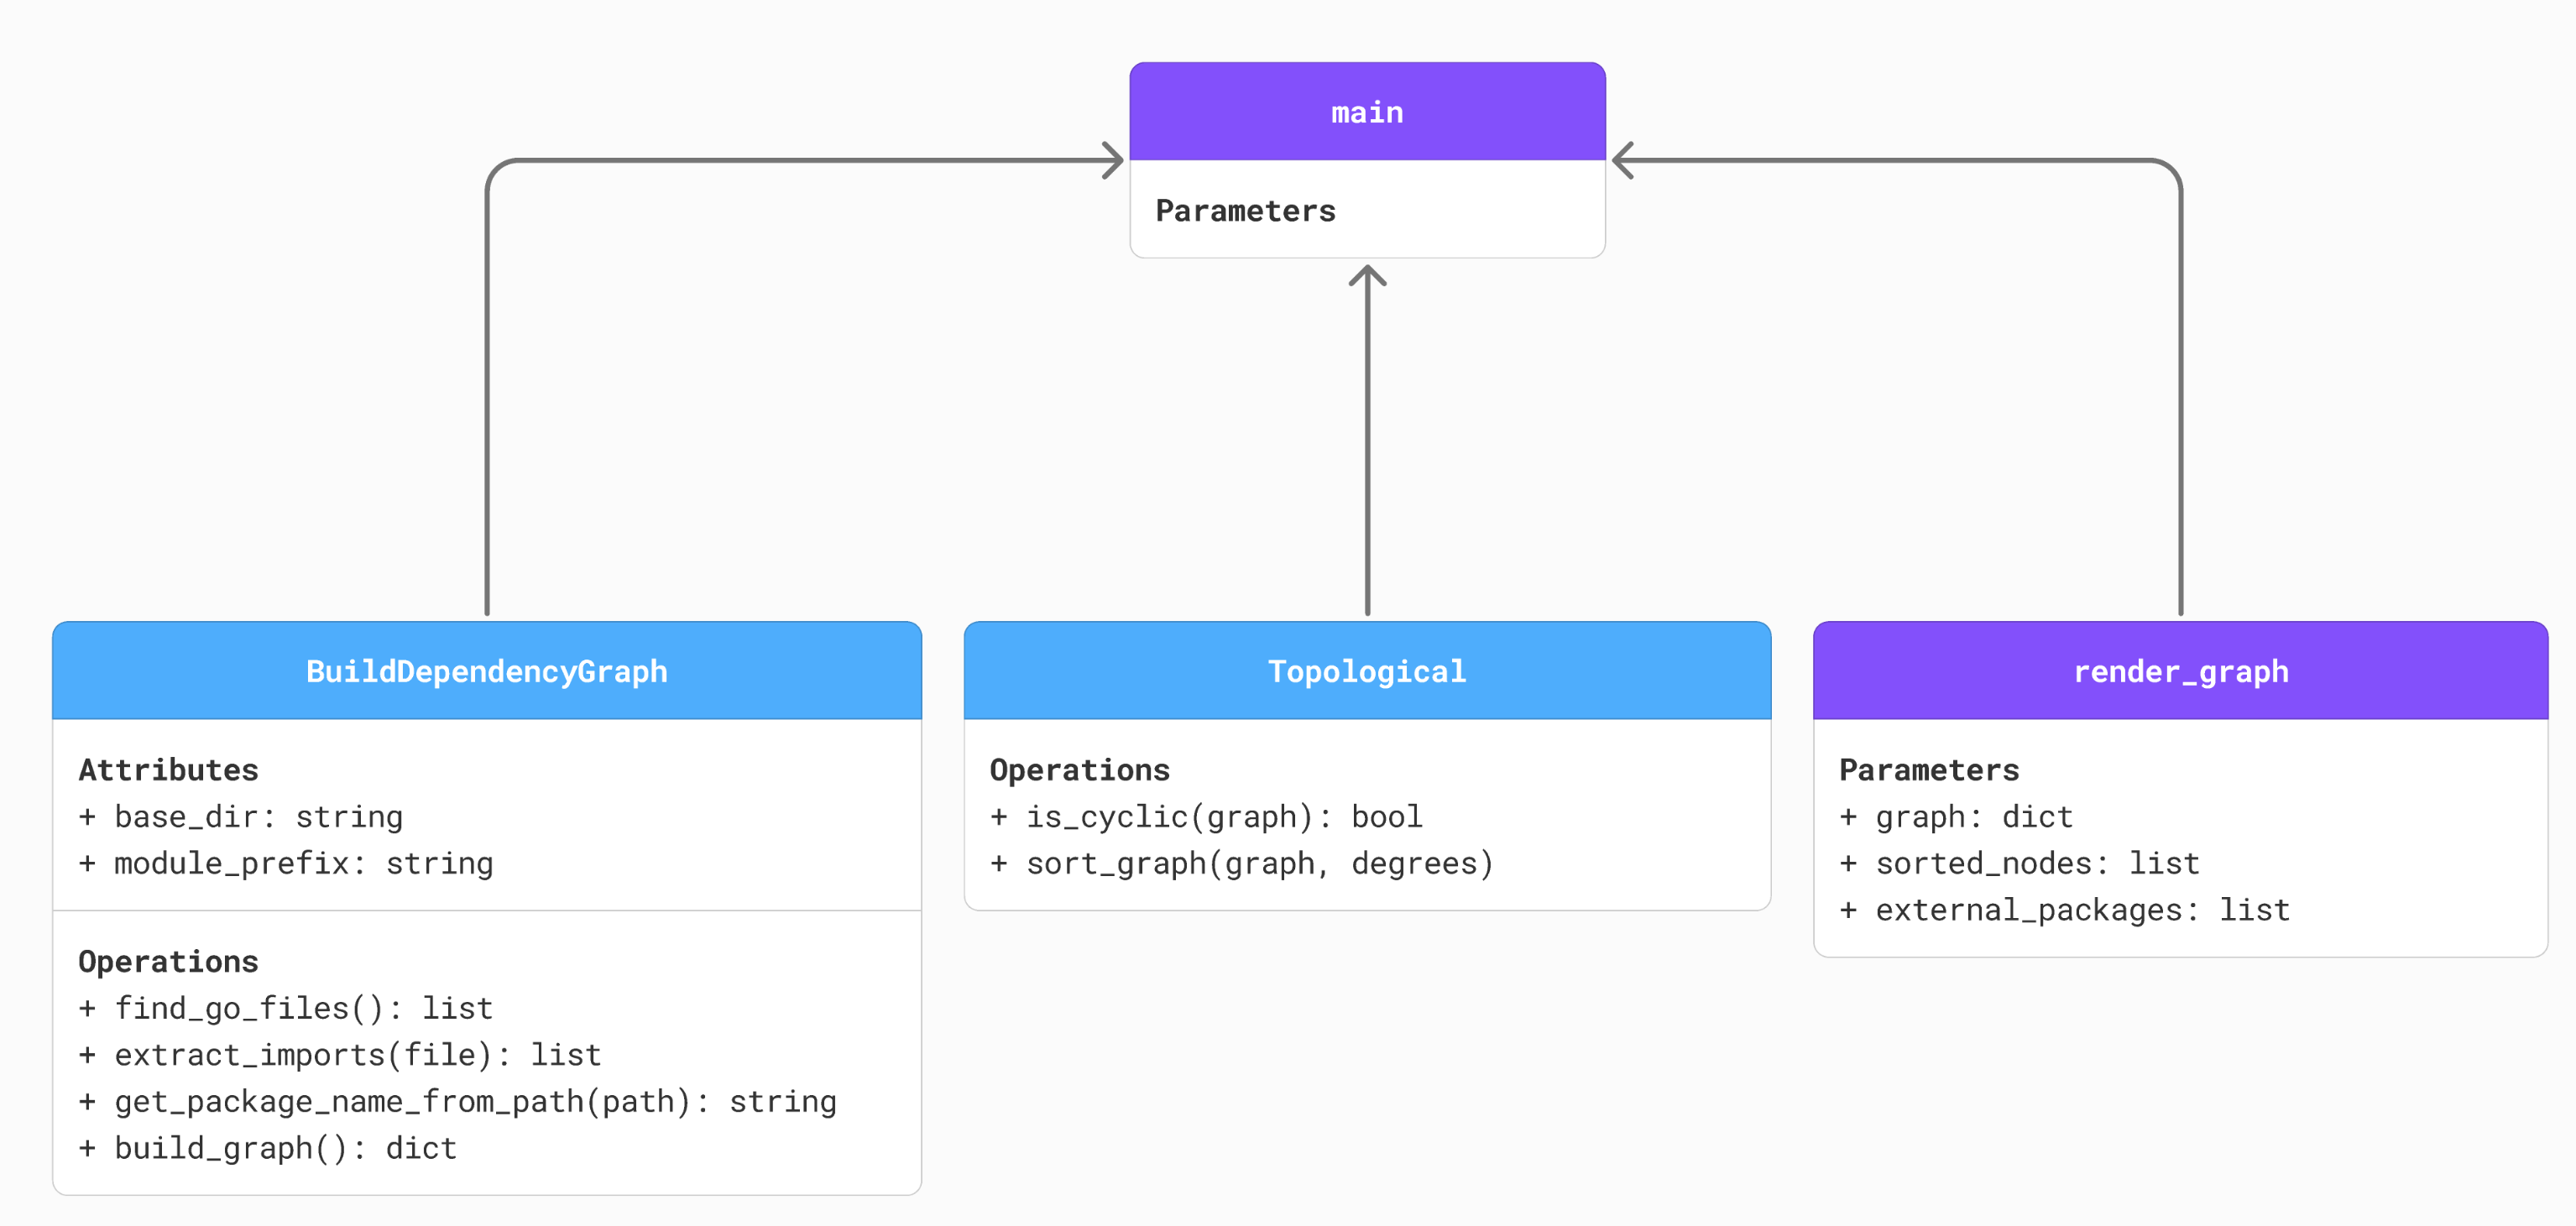
\includegraphics[width=0.9\textwidth]{images/diagrama_classes.png}
    \caption{Fluxo de execução: Extração, Processamento e Visualização.}
  \end{figure}
\end{frame}

% ---------------------------------------------------------------
% SLIDE 6: Resultados: Padrões de Arquitetura
% ---------------------------------------------------------------
\begin{frame}
  \frametitle{Resultados: Padrões de Arquitetura Identificados}

  \begin{columns}[T]
    \begin{column}{0.32\textwidth}
      \centering
      \textbf{Framework (Hub)}\\
      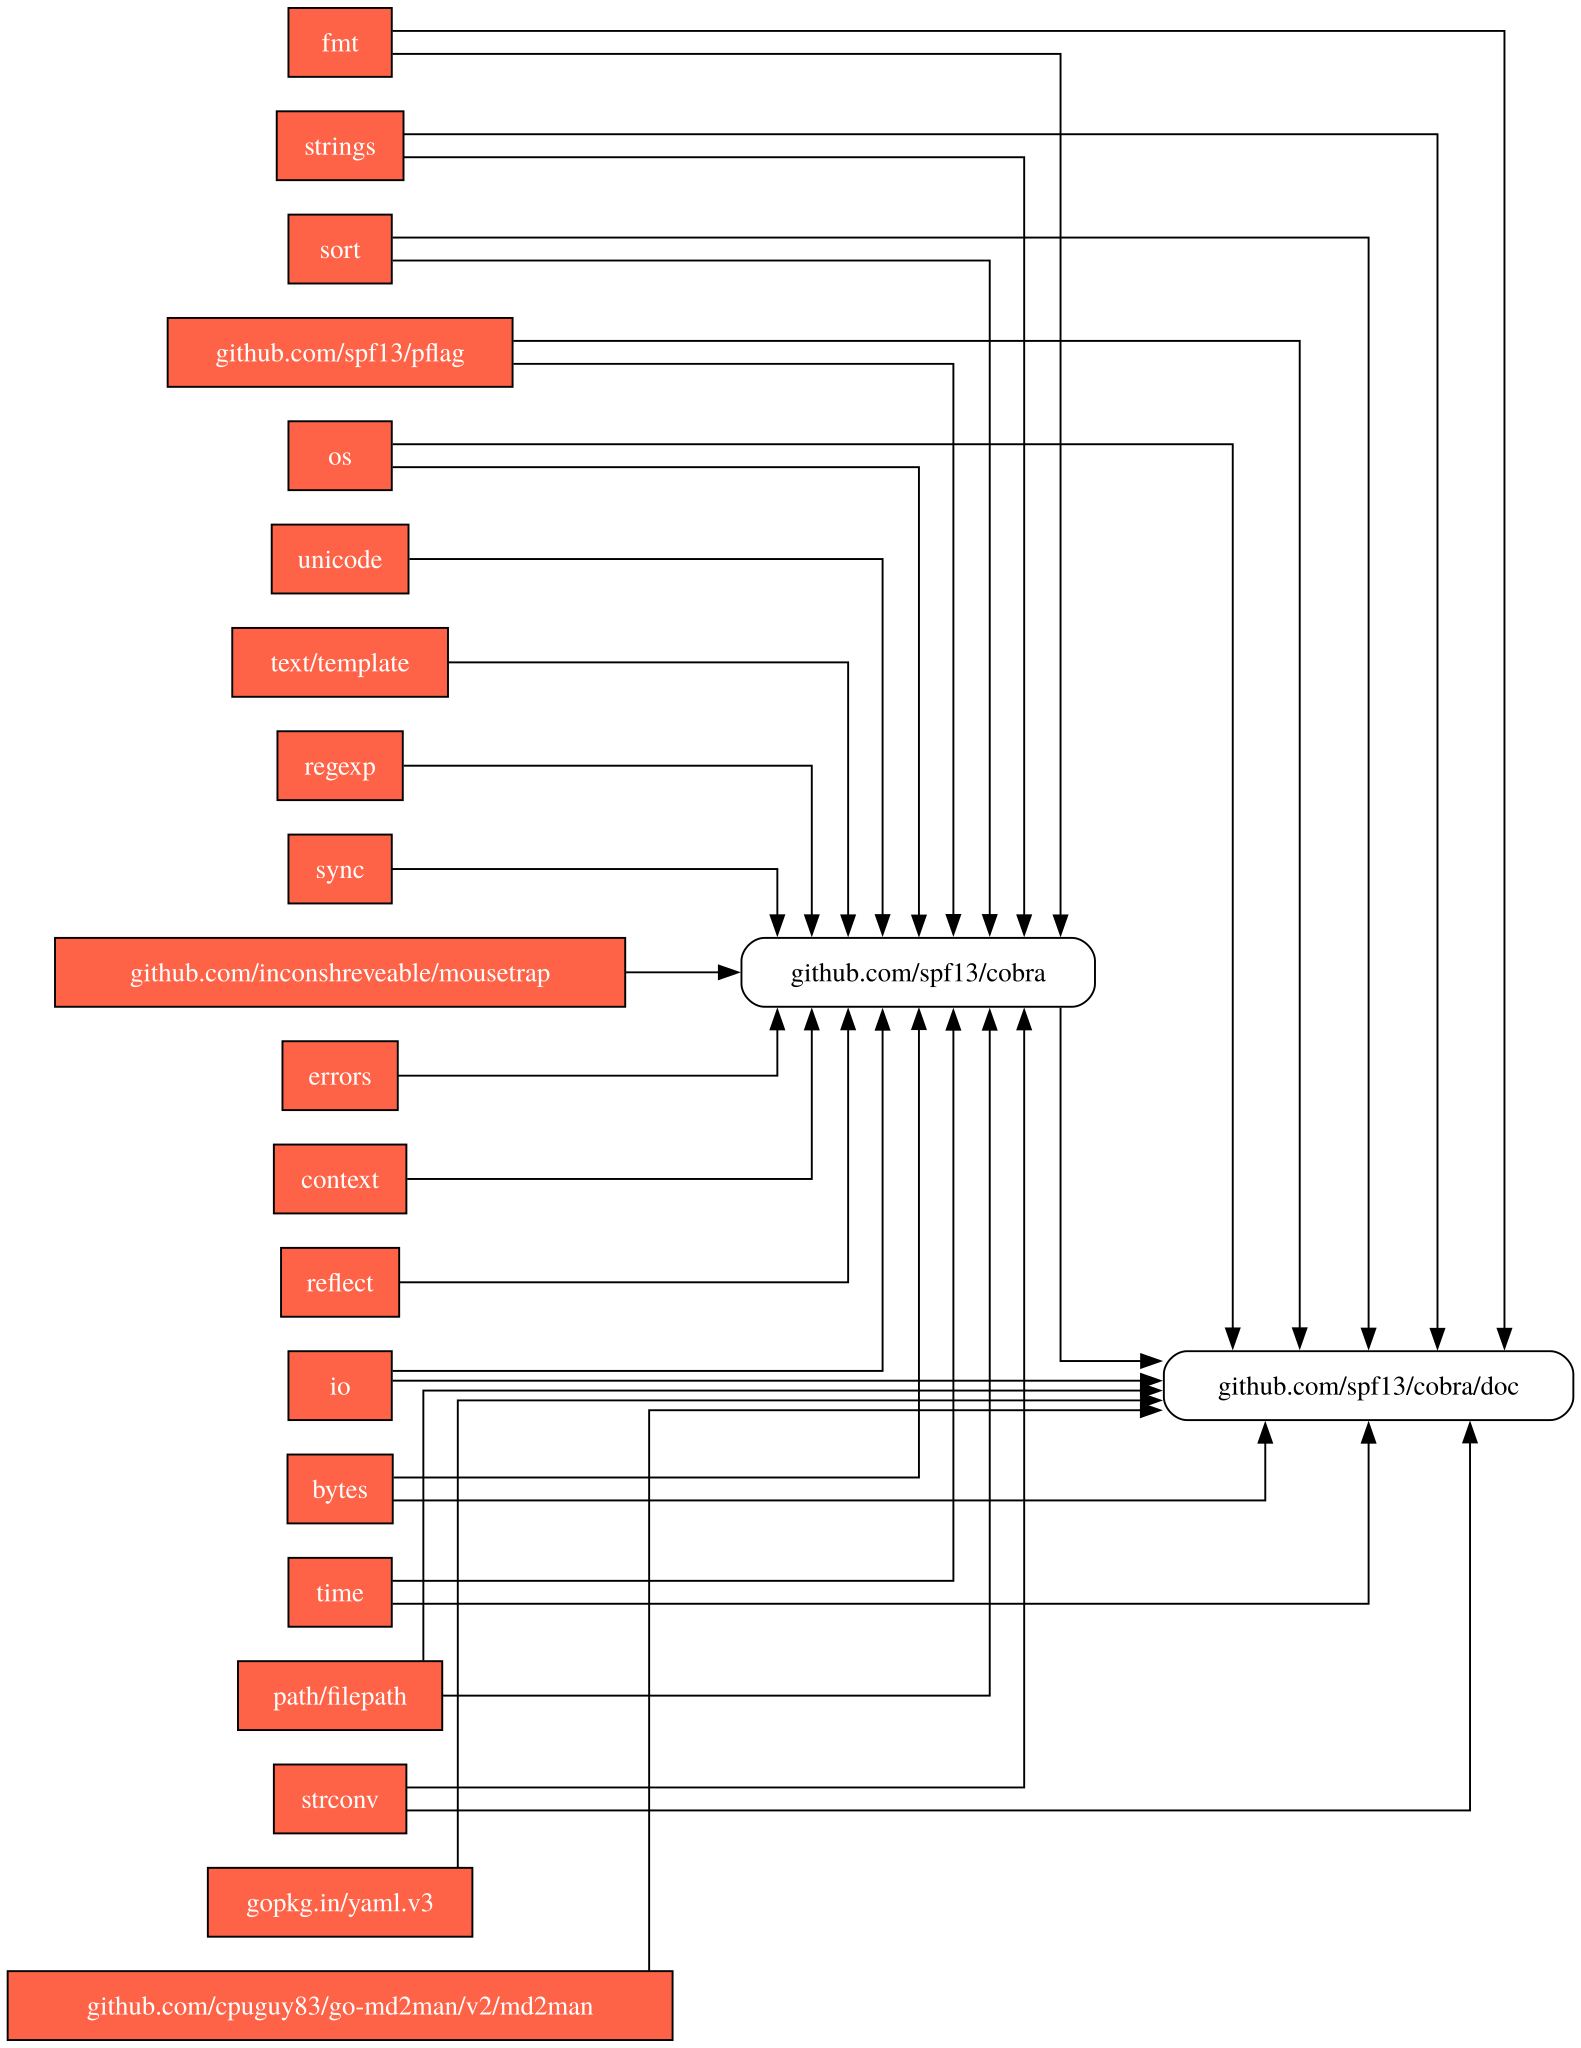
\includegraphics[width=\textwidth]{images/github.com_spf13_cobra.png}
      \tiny
      Um pacote central (`cobra`) oferece a funcionalidade principal.
    \end{column}
    \begin{column}{0.32\textwidth}
      \centering
      \textbf{Aplicação (Consumidor)}\\
      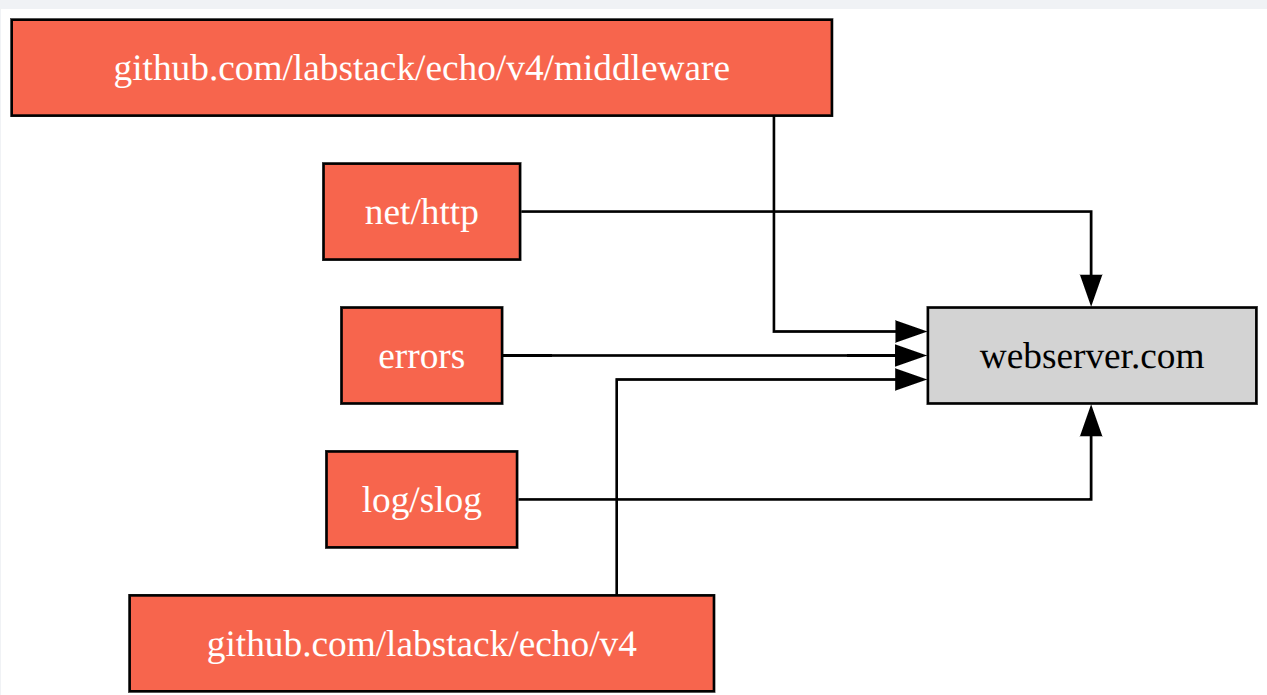
\includegraphics[width=\textwidth]{images/webserver.png}
      \tiny
      Um pacote principal (`webserver.com`) consome múltiplas bibliotecas.
    \end{column}
    \begin{column}{0.32\textwidth}
      \centering
      \textbf{Bindings (Wrapper)}\\
      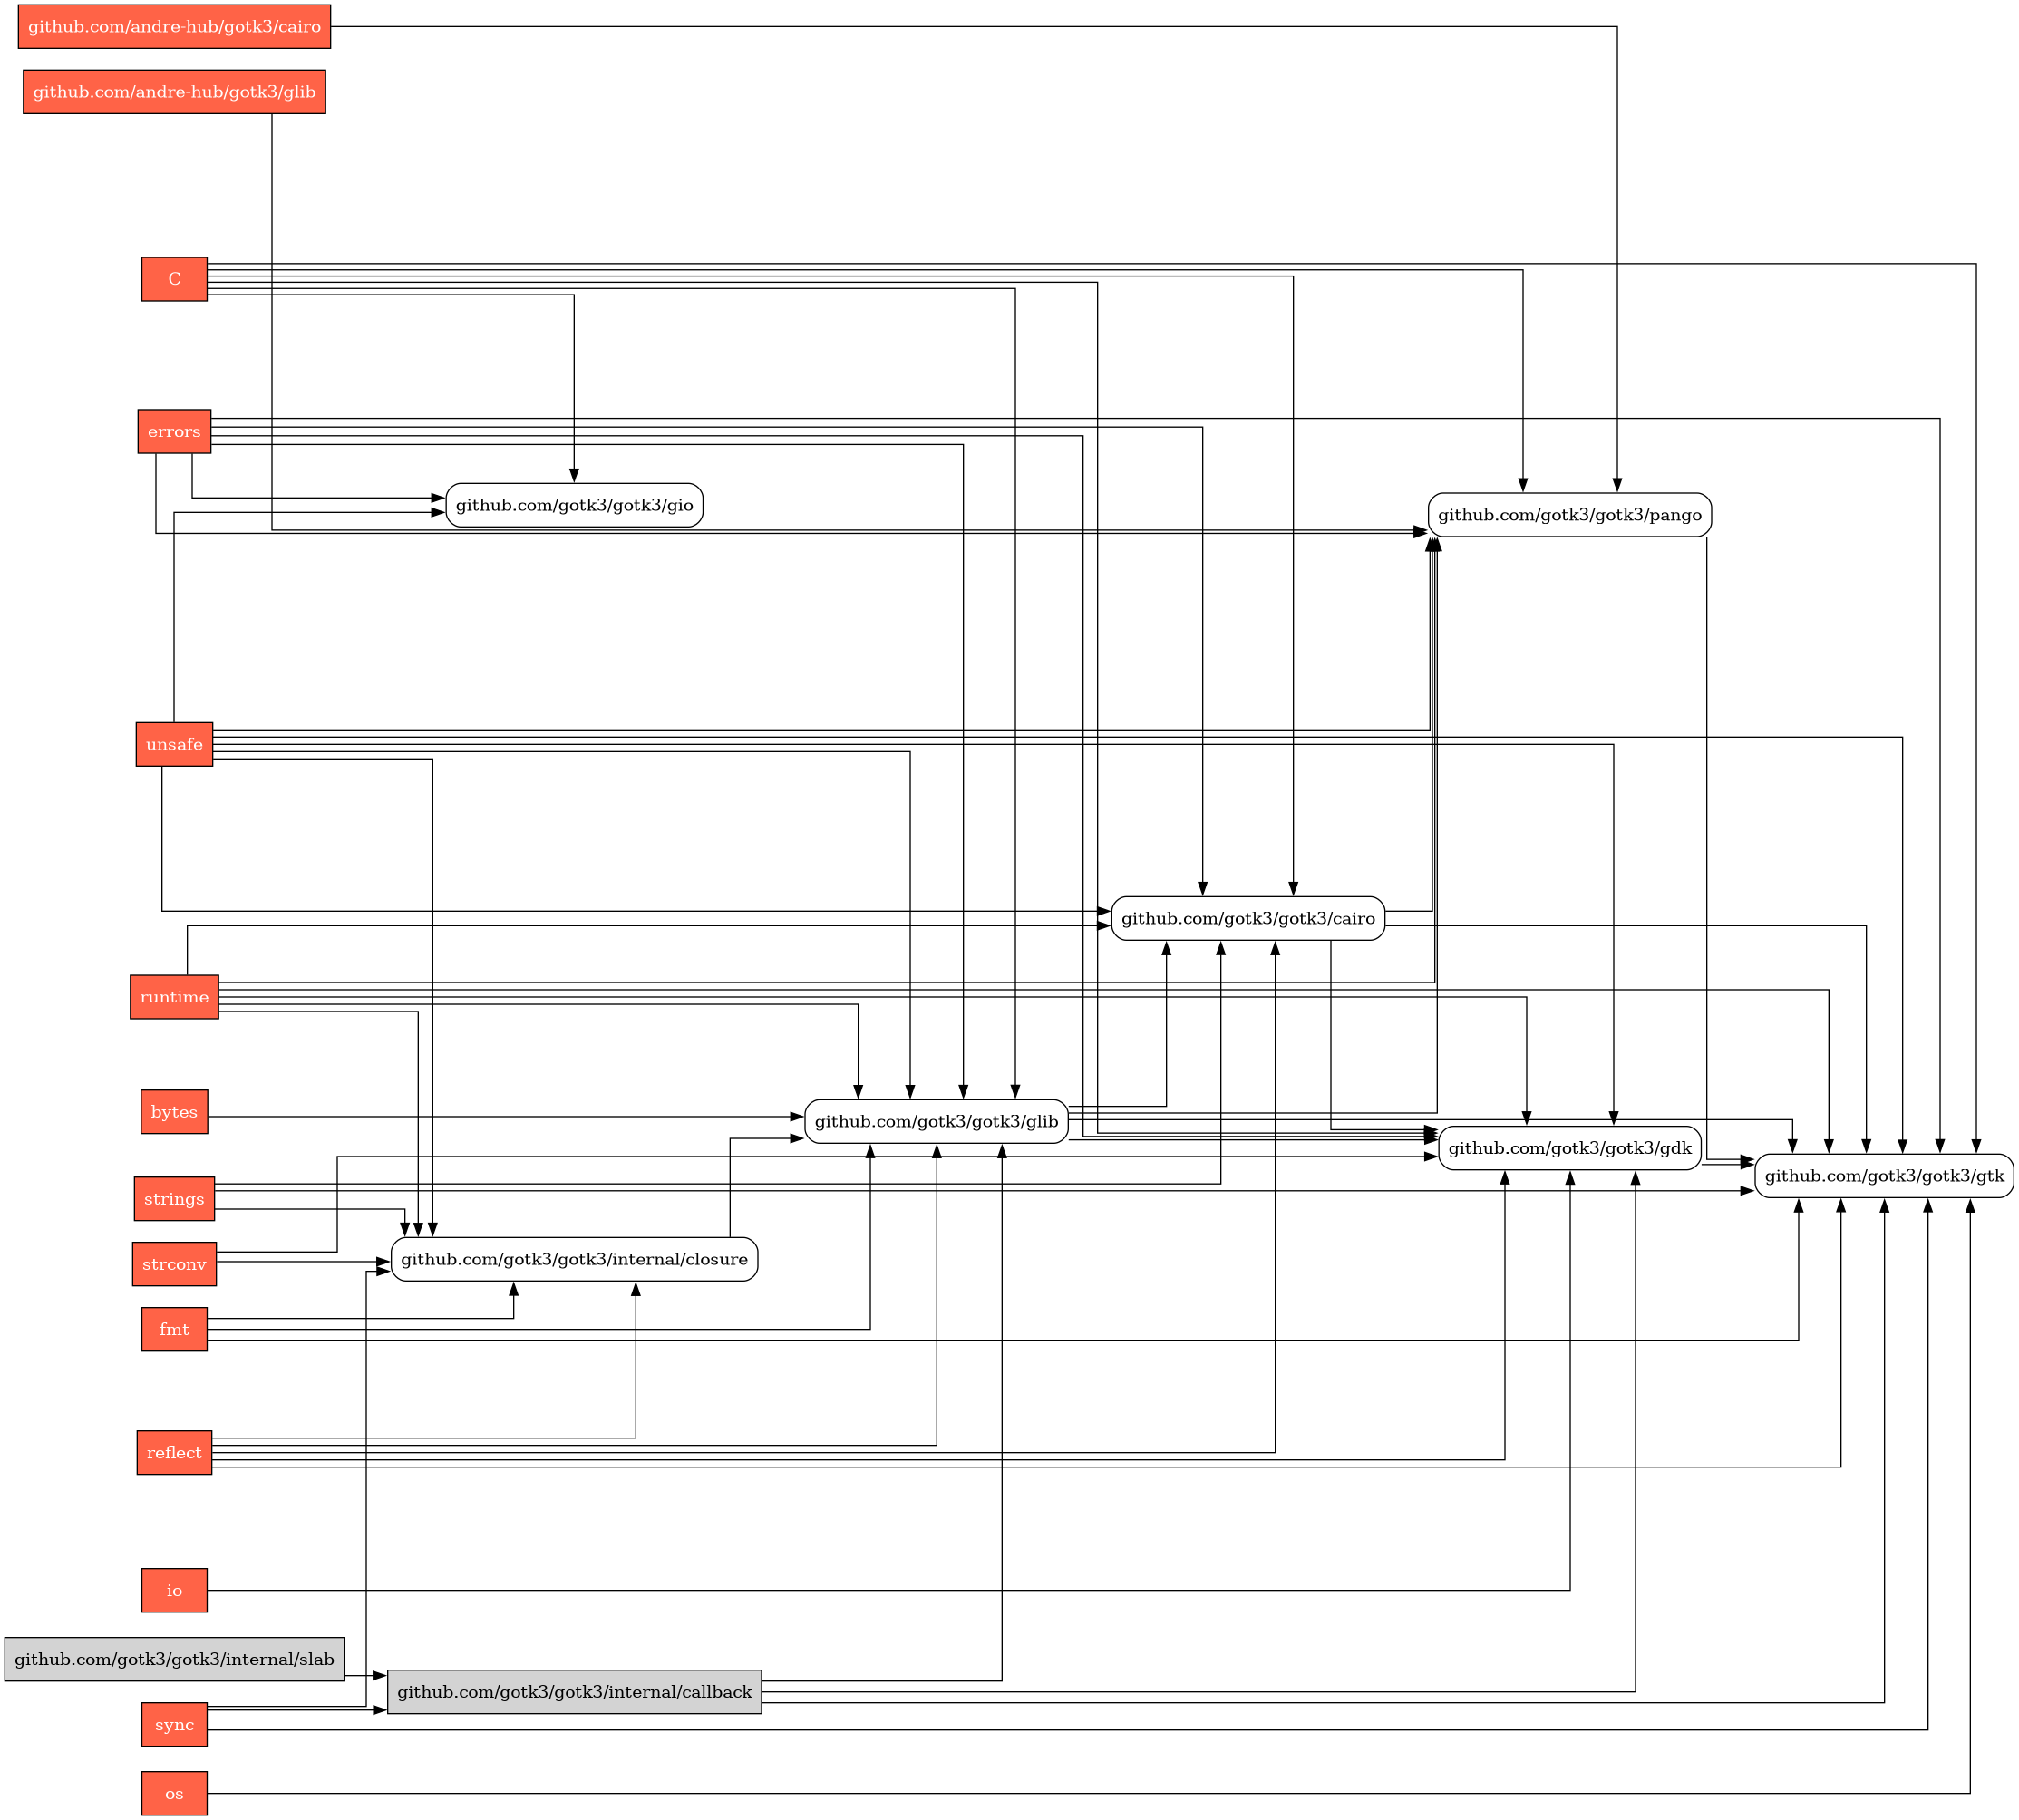
\includegraphics[width=\textwidth]{images/gotk3.png}
      \tiny
      Muitos pacotes pequenos que espelham uma biblioteca C externa (GTK3).
    \end{column}
  \end{columns}
\end{frame}

% ---------------------------------------------------------------
% SLIDE 7: Conclusão
% ---------------------------------------------------------------
\begin{frame}
  \frametitle{Conclusão e Trabalhos Futuros}

  \textbf{Conclusões}
  \begin{itemize}
      \item A modelagem de dependências como um grafo é uma abordagem eficaz e visual para entender a arquitetura de software.
      \item A ferramenta desenvolvida valida a ordem de compilação, detecta ciclos e revela padrões de design de forma automatizada.
      \item A visualização em camadas facilita a identificação de componentes críticos e o fluxo de dependências.
  \end{itemize}
  \vspace{1cm}

  \textbf{Trabalhos Futuros}
  \begin{itemize}
      \item \textbf{Parser Avançado (AST):} Aumentar a precisão da extração de dependências.
      \item \textbf{Integração com IDEs:} Fornecer feedback sobre ciclos em tempo real para o desenvolvedor.
  \end{itemize}

\end{frame}

% ---------------------------------------------------------------
% SLIDE 8: Agradecimento
% ---------------------------------------------------------------
\begin{frame}
  \vfill
  \centering
  \huge{\textbf{Obrigado!}}
  \vspace{1cm}
  \Large{Perguntas?}
  \vfill
\end{frame}


\end{document}
